\section{Regularization of detector unfolding}
\label{sec:regularization}

\emph{
This study into the need and possible implementation of detector unfolding was performed with the differential cross sections of the $\hgg$ channel in mind.
% 
As the arguments and circumstances of this study have not changed since it was performed, the conclusions were extrapolated to the combination performed in Section~\ref{sec:diffxs}.
% 
The text, arguments and figures in this section closely follow the original study in Ref.~\cite{AN-17-041}.
}

Event observables are generally reconstructed with some finite resolution.
% 
When considering a binned spectrum in an observable, this finite resolution can lead to events being reconstructed in a different bin than the one to which the true observable belongs, a phenomenon known as bin-to-bin migrations.
% 
Since theory predictions generally concern spectra before detector folding, there is a need to determine a best estimate of true observables based on the reconstructed observables.
% 
The procedure of undoing the detector folding due to finite resolution is called unfolding.


In matrix form, detector folding can be written as
% 
\begin{linenomath*}
\begin{equation}
K \vec{\mu}_{\text{gen}} = \vec{\mu}_{\text{reco}}
\,,
\end{equation}
\end{linenomath*}
%
where $K$ is the response matrix, $\vec{\mu}_{\text{gen}}$ is a vector of the fiducial cross sections at the generator level and $\vec{\mu}_{\text{reco}}$ the observed spectrum.
% 
Naively one could estimate $K$ using Monte Carlo simulations and find $\vec{\mu}_{\text{gen}}$ by simply inverting:
% 
\begin{linenomath*}
\begin{equation}
\vec{\mu}_{\text{gen}} = K^{-1} \vec{\mu}_{\text{reco}}
\,.
\end{equation}
\end{linenomath*}
%
In practice, simple inversion of $K$ often leads to strongly oscillating components in $\vec{\mu}_{\text{gen}}$ due to unreasonably large weights on bins with few events. In the unfolding problem one is not interested in the exact solution, but in the most likely physical solution. Finding this solution is done by adding a regularization term to the overall likelihood scan:
% 
\begin{linenomath*}
\begin{equation}
q(\vec{\mu}_{\text{gen}})_R = q(\vec{\mu}_{\text{gen}}) + \tau \, || C \cdot \vec{\mu}_{\text{gen}} ||
\,,
\label{eq:likelihoodaddition}
\end{equation}
\end{linenomath*}
% 
where $C$ is some matrix and $\tau$ is the regularization strength. In the case of unfolding signal strength for $\hgg$ differential cross sections, $C$ is chosen to be the second derivative matrix (also curvature matrix):
% 
\begin{linenomath*}
\begin{equation}
C = \left[
\begin{array}{c c c c c c}
-1 & 1 & 0 & 0 & \dots &  \\
1 & -2 & 1 & 0 & \dots &  \\
0 & 1 & -2 & 1 & \dots &  \\
  & \cdots &   &   & \cdots &  \\
  & \cdots &   & 1 & -2 & 1 \\
  & \cdots &   &   & 1 & -1
\end{array}
\right]
\,.
\end{equation}
\end{linenomath*}
%
Constraining the second derivative of the signal strengths over bins means the highly oscillating components of the unregularized solution will be suppressed.
% 
From a physical point of view this makes sense, as large bin-to-bin variations are not expected.


\subsection{The effect of $\tau$ on the unfolded spectrum}

With $C$ given, the effect of $\tau$ on the unfolded spectrum is investigated by scanning over a range of values for $\tau$.
% 
The contribution to the likelihood due to the regularization, $|| C \mu_{\text{gen}} ||$, is plotted against the likelihood one would obtain without a regularization term $q(\vec{\mu}_{\text{gen}})$ (also called the residual term).
% 
One expects to see a clear boundary at the point where highly weighted bins with low event count are adequately suppressed~\cite{Hansen:LShape}.
% 
An example of such a shape is given in Fig.~\ref{fig:expectedlshape}.

\begin{figure}[ht]
 \begin{center}
   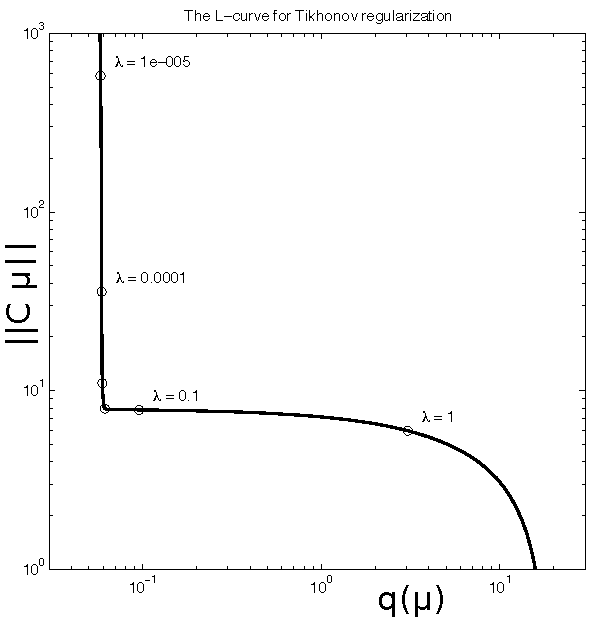
\includegraphics[width=\halflinewidth]{img/differentials/regularization/Lshape2.pdf}
   \caption{ Expected shape of the regularization contribution vs. the residual term. Taken from Ref.~\cite{Hansen:LShape} (adapted). }
   \label{fig:expectedlshape}
 \end{center}
\end{figure}



The regularization term in Eq.~(\ref{eq:likelihoodaddition}) is implemented in the likelihood of the $\njets$ spectrum, which is known to have large off-diagonal components.
% 
As the expected spectrum has zero curvature by construction, the ``L-shape'', as demonstrated in Fig.~\ref{fig:expectedlshape}, is computed for a high number of toys rather than the Asimov dataset.
% 
The L-shape is also computed for the $\njets$ spectrum extracted from data obtained by the CMS detector in 2016, corresponding to an integrated luminosity of $35.8$\fbinv.
% 
As an example, Fig.~\ref{fig:regularizationtoystudy} shows the L-shape and the corresponding unfolded regularized spectra for data (first row) and for a toy (second row).
% 
The transition between under- and overregularization is smooth, which indicates the suppression of curvature is seemingly ineffective at suppressing oscillations due to highly weighted bins with low event count while preserving statistical fluctuations inherent to the observation.
% 
This conclusion is made decisive by computing an aggregate L-shape for a number of toys, as is done in Fig.~\ref{fig:median}.
% 
Also for a large number of toys, there is no clear value of $\tau$ at which oscillations due to underregularization are suppressed.
% 
While not shown here, the same observations are made for the regularization of the $\pth$ spectrum.
%
It is concluded that no clear criterion for adding a regularization term to the likelihood is found, and as such no regularization term is added to the likelihood.


\begin{figure}[ht]
 \begin{center}
   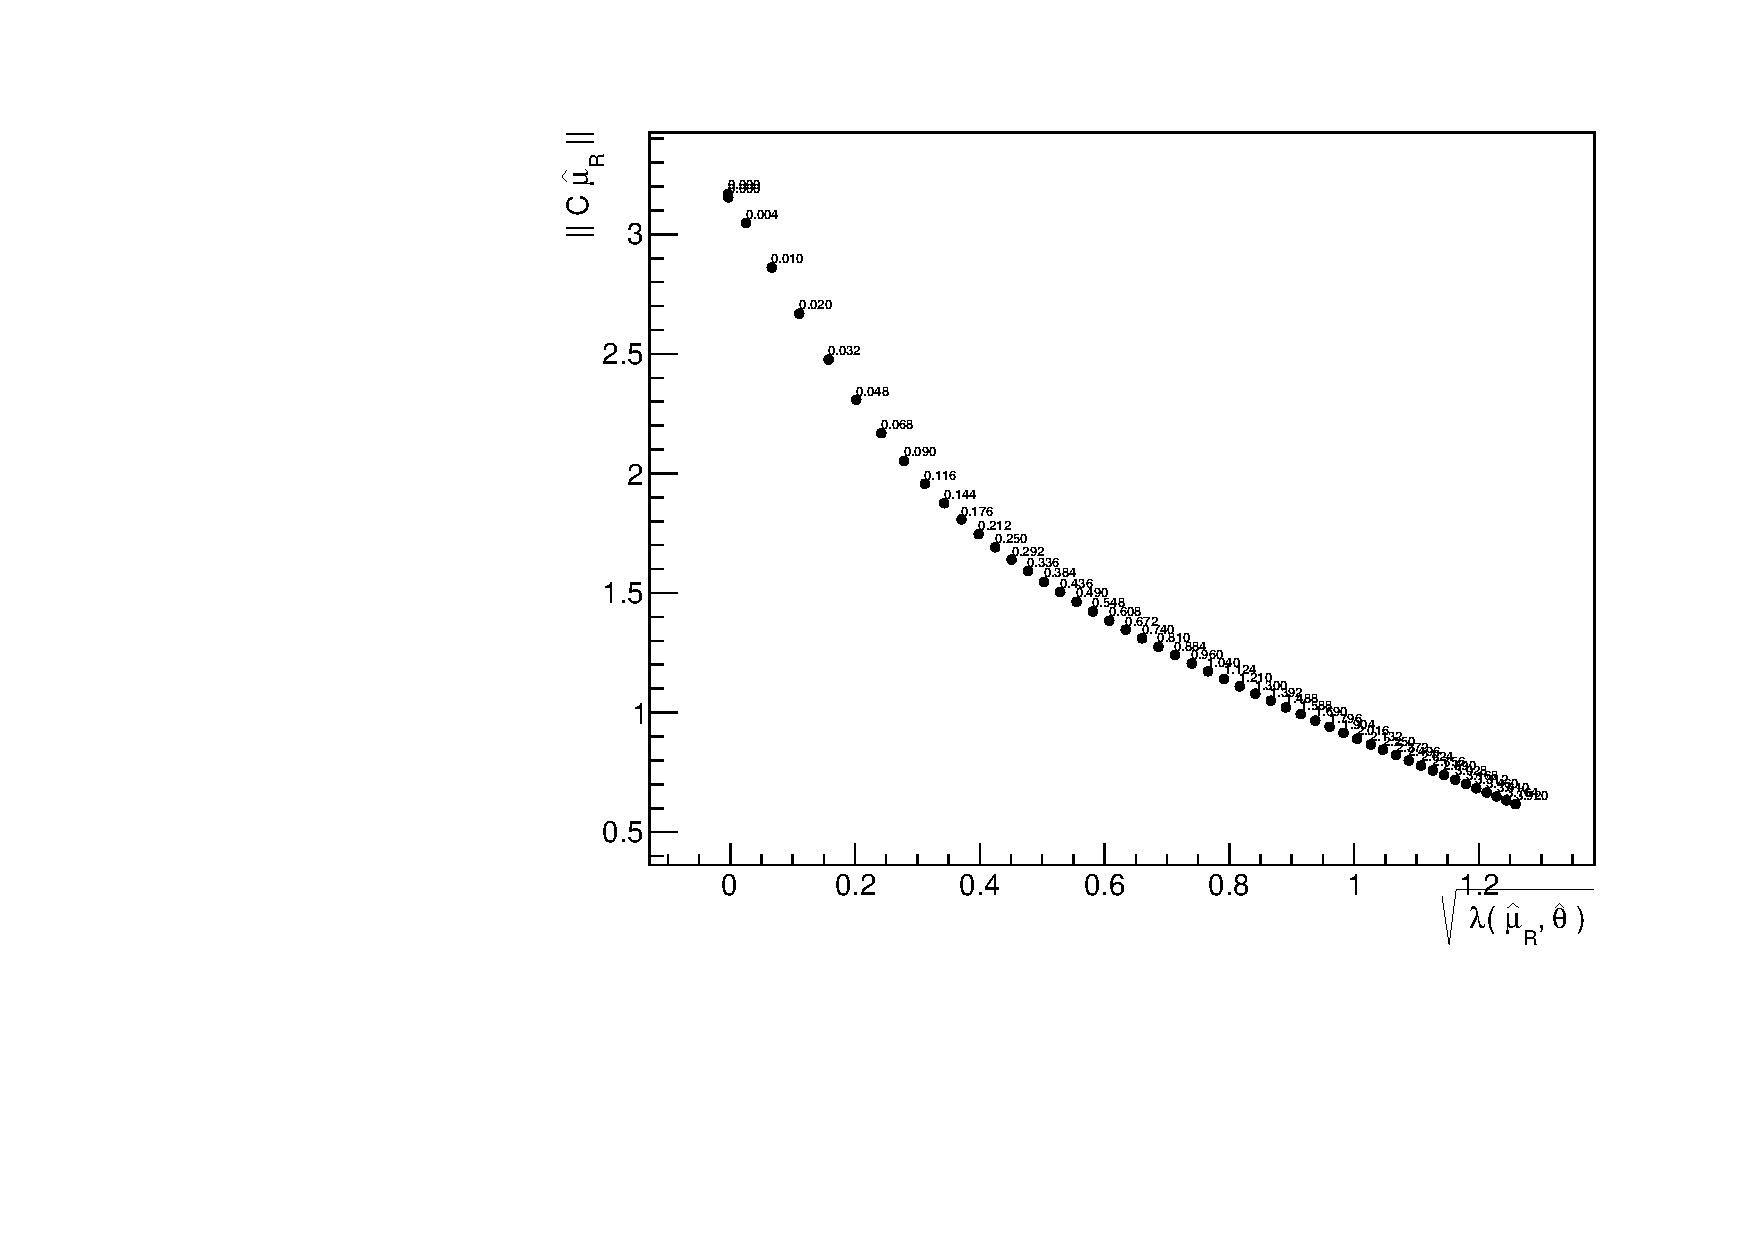
\includegraphics[width=\halflinewidth]{img/differentials/regularization/Lshape.pdf}
   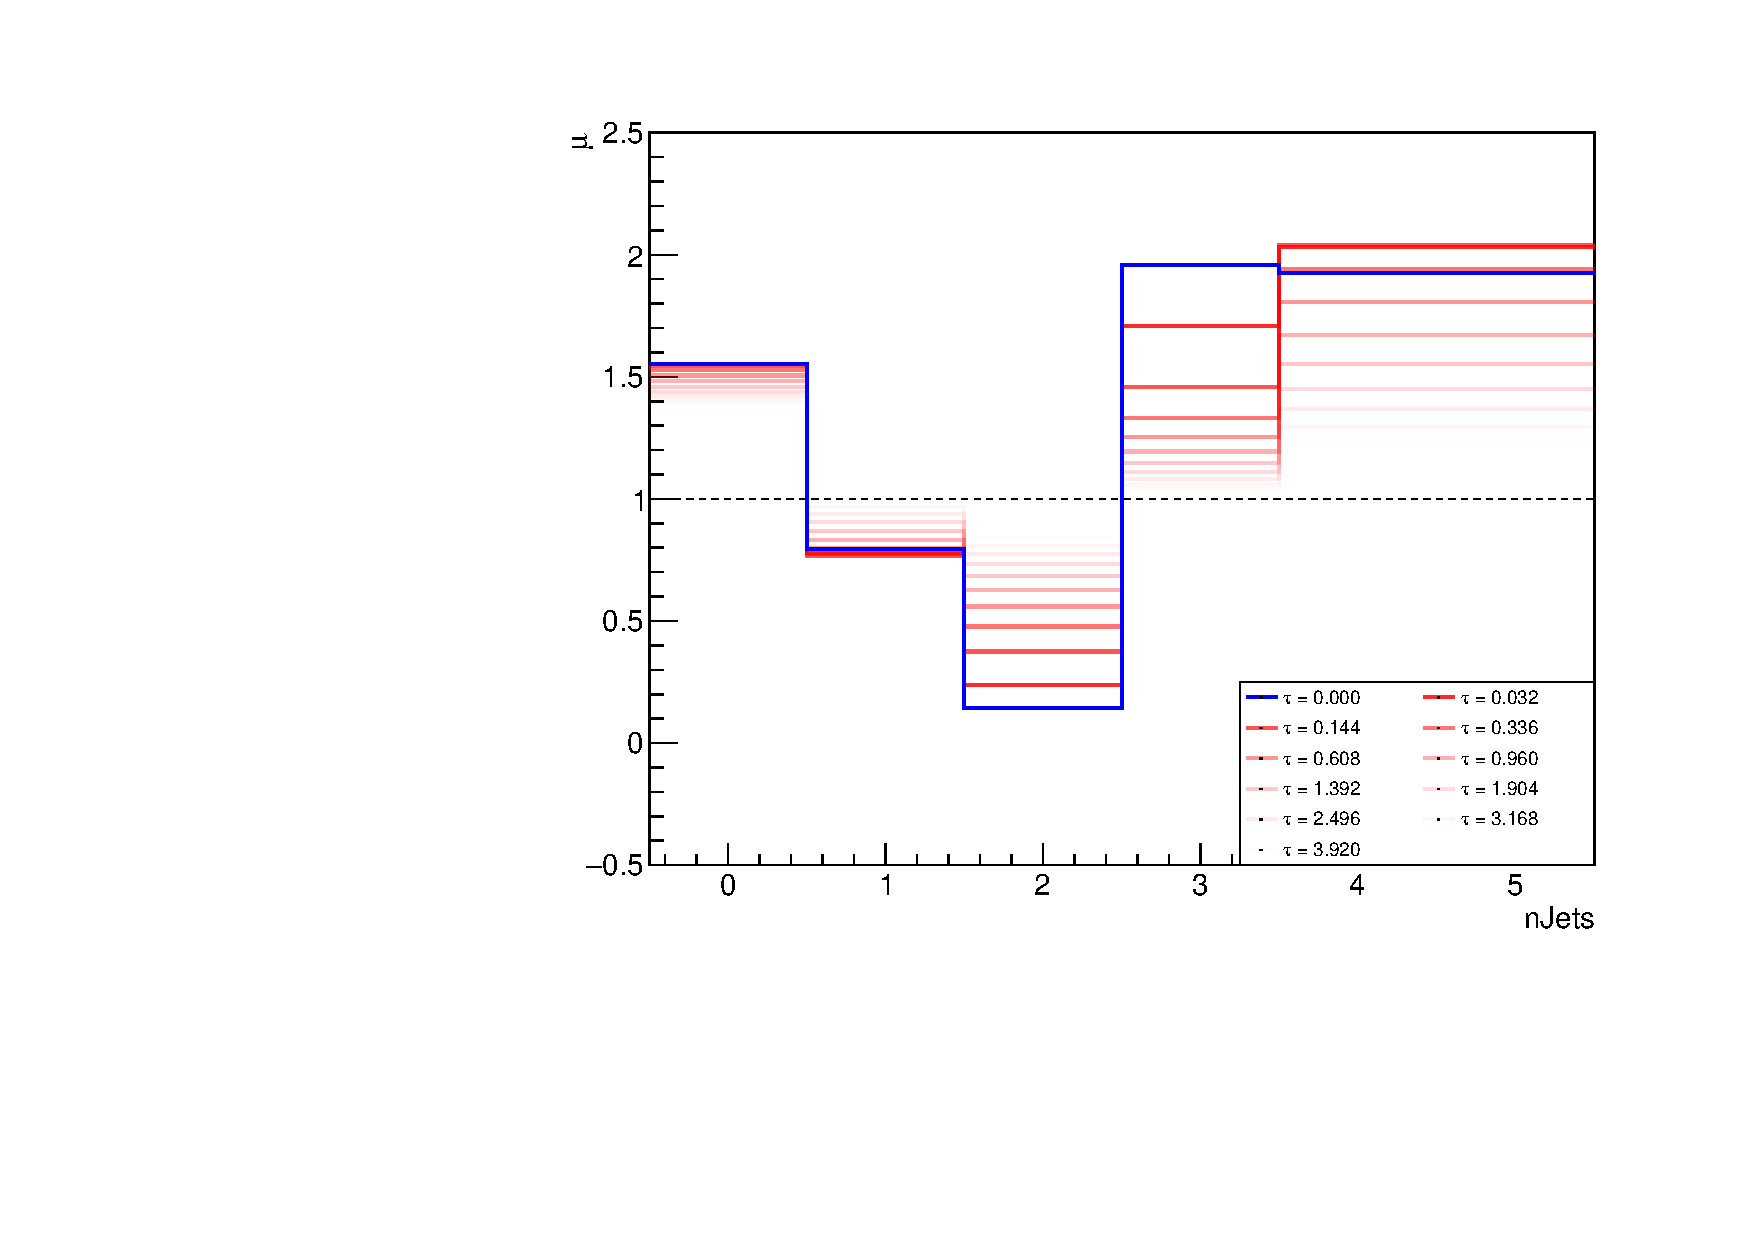
\includegraphics[width=\halflinewidth]{img/differentials/regularization/SeveralUnfoldedSpectra.pdf}
   \\[-10pt]
   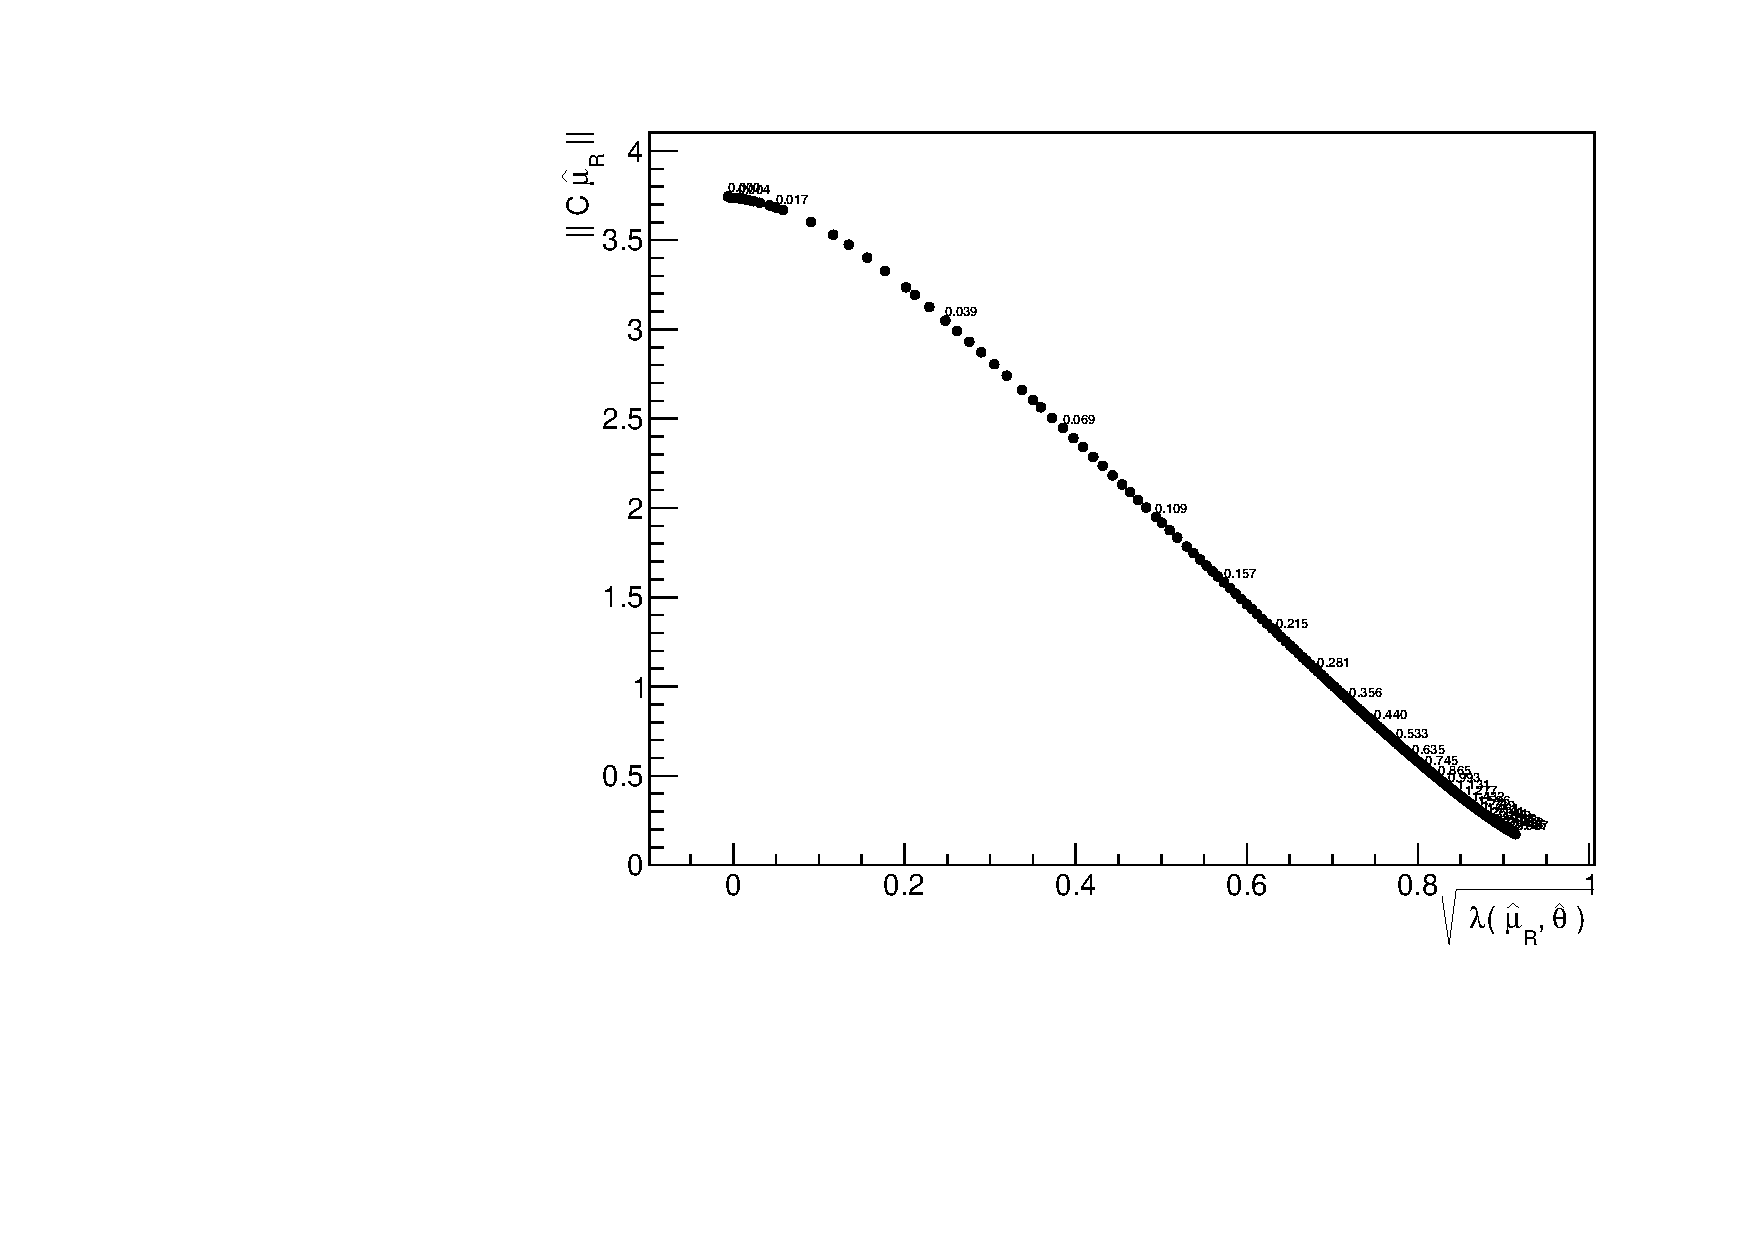
\includegraphics[width=\halflinewidth]{img/differentials/regularization/seed7003_Lshape.pdf}
   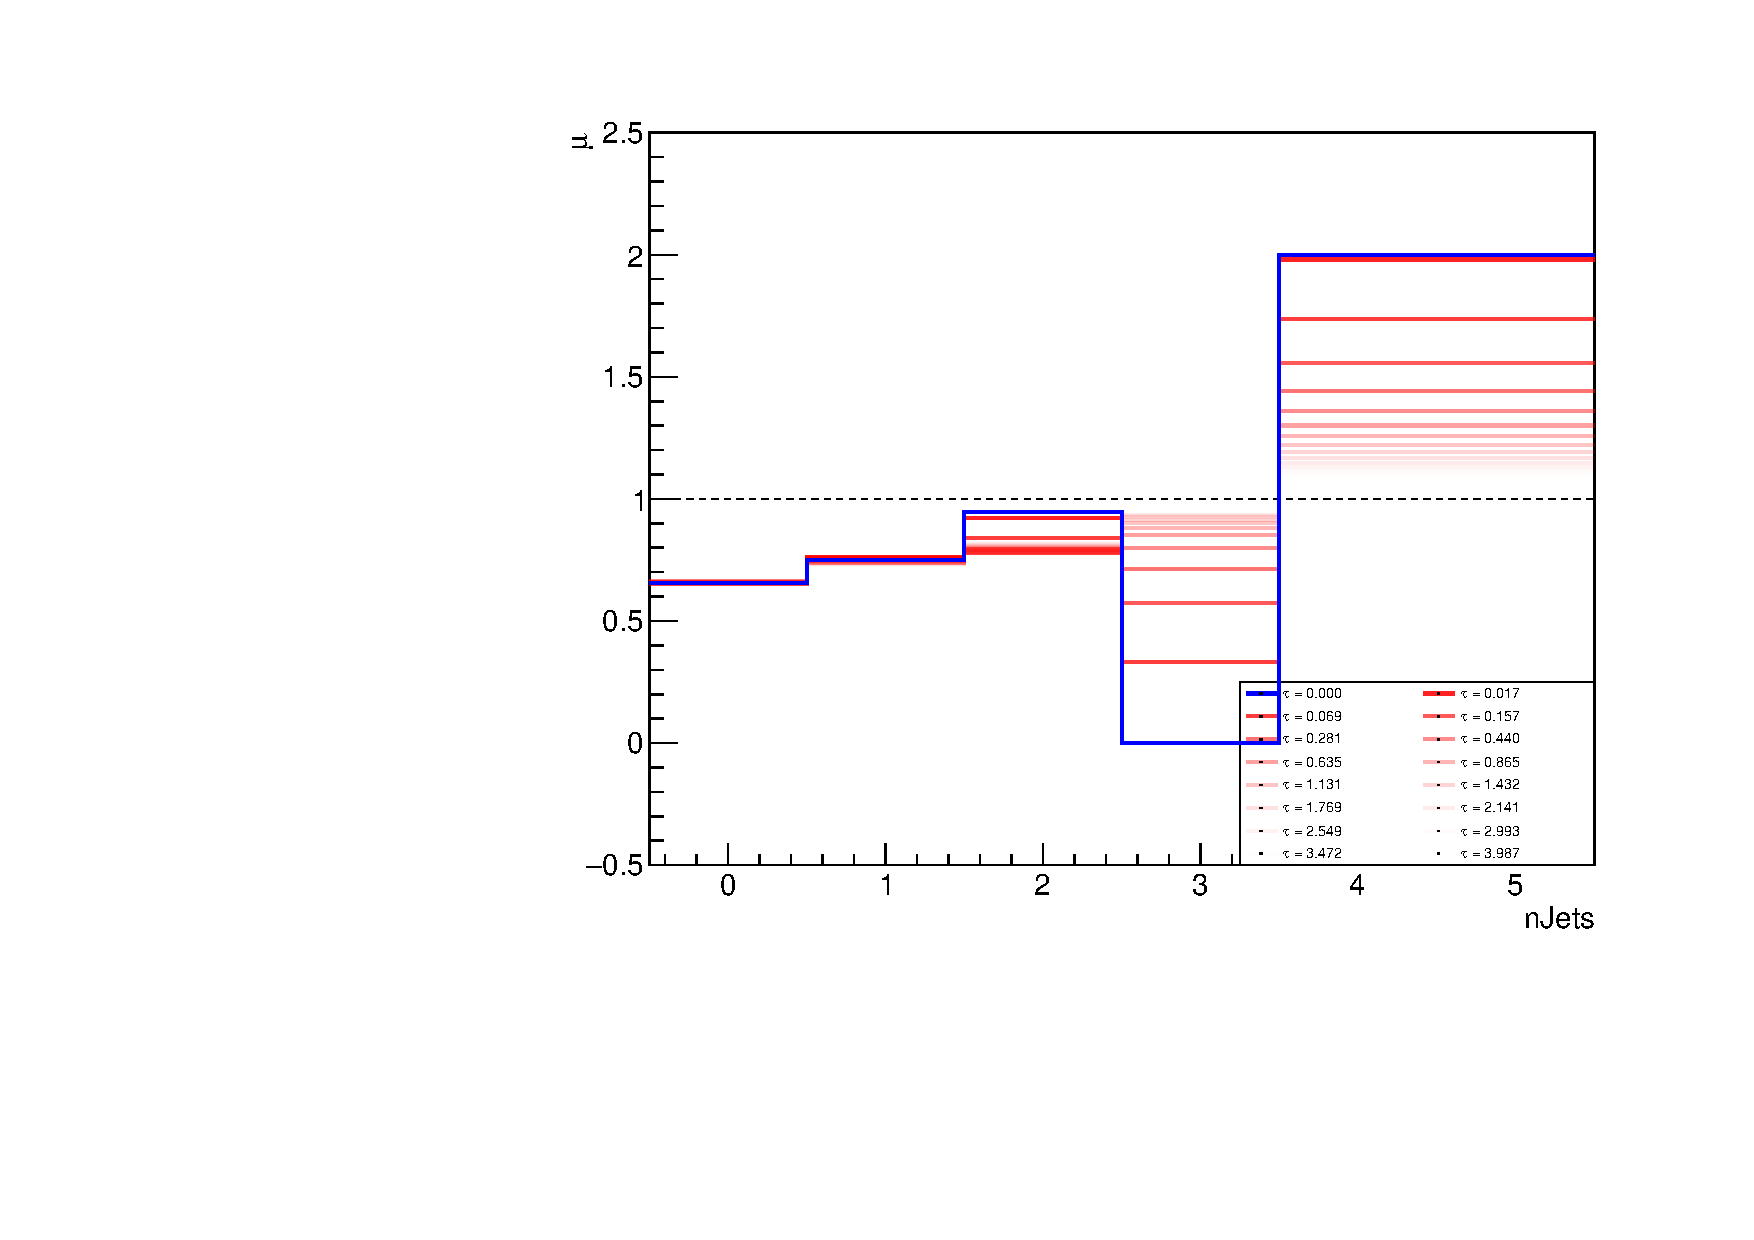
\includegraphics[width=\halflinewidth]{img/differentials/regularization/seed7003_SeveralUnfoldedSpectra.pdf}
   \caption{The ``L-shape'' plots (left) and the unfolded spectra (right) for various regularization strengths for the number-of-jets spectrum for data (first row) and a toy (second row).}
   \label{fig:regularizationtoystudy}
 \end{center}
\end{figure}


\begin{figure}[ht]
 \begin{center}
   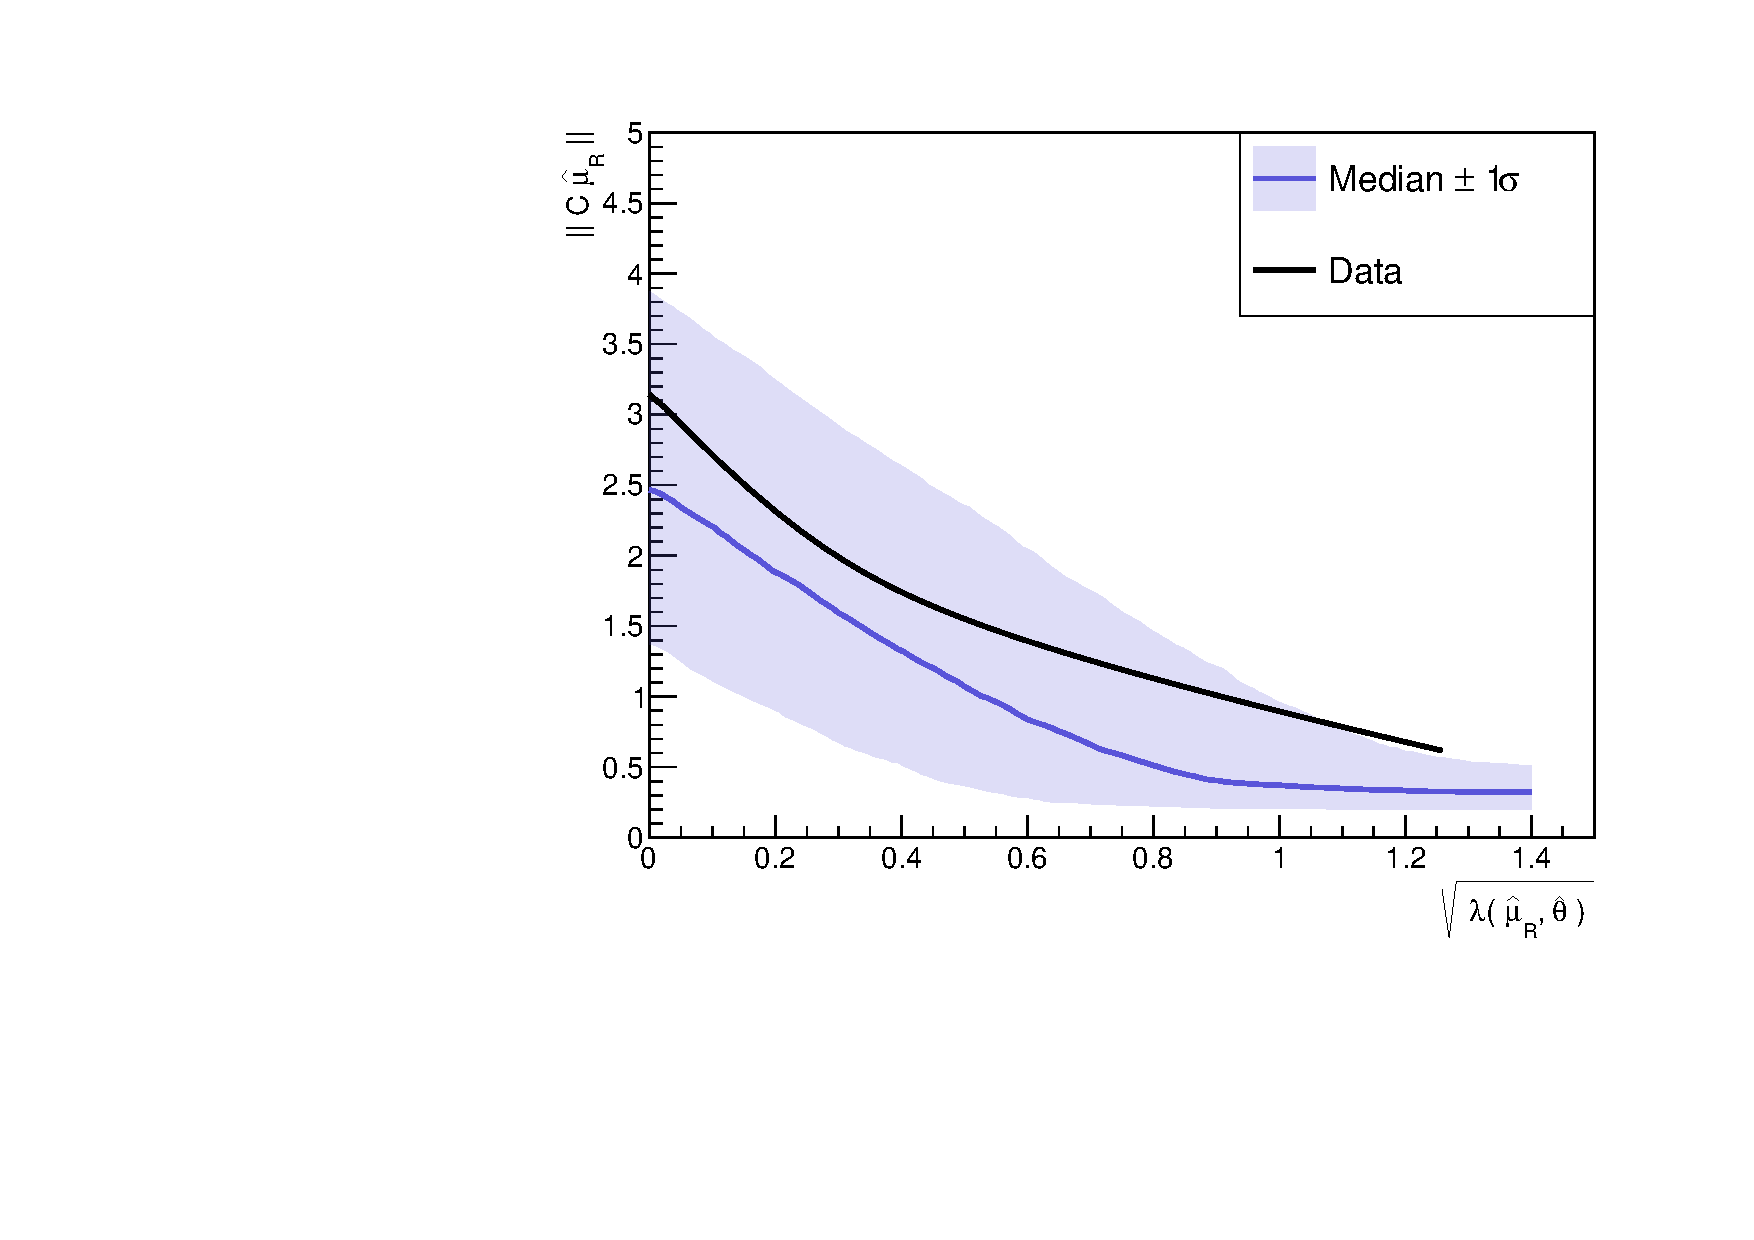
\includegraphics[width=\halflinewidth]{img/differentials/regularization/combinedLshapes_Median_better.pdf}
   \caption{ The median L-shape of 1000 toys, and the L-shape of the measured number-of-jets spectrum. }
   \label{fig:median}
 \end{center}
\end{figure}

